% ============================================================
% トランジスタを用いた回路 本文
% 原本: トランジスタを用いた回路 20260727.docx
% 担当の先生はこのファイルと figures/ だけを編集してください。
% 図のラベルは fig:transistor-○○ の形にしてください（他テーマとの重複防止）。
% ============================================================
\graphicspath{{contents/04_transistor/figures/}}

\experimenttitle{トランジスタを用いた回路}

% ============================================================
\section{目的}

トランジスタは，小さな電気信号を用いてより大きな電流を制御できる電子素子であり，信号の増幅やスイッチングなど，さまざまな電子回路に広く利用されています。本実験では，トランジスタを用いてファンを駆動する回路を作製し，小さな入力によって負荷に流れる大きな電流を制御できることを確認します（\cref{fig:transistor-overview}）。さらに，入力電圧を変化させたときの電流や出力電圧を測定し，トランジスタの基本的な特性について理解します。

\begin{figure}[htbp]
  \centering
  \vspace{5mm}
  % 本実験の概要図（TikZ で作成。原本にはない図）
  \begin{tikzpicture}[
      font=\small,
      lbl/.style={font=\sffamily\gtfamily\small, align=center},
      small/.style={-latex, line width=0.6pt, EGMain!70},
      big/.style={-{Latex[length=3.2mm,width=3.2mm]}, line width=3pt, EGWarn!80},
    ]
    % ---- 入力：乾電池 ----
    \begin{scope}[shift={(0,0)}]
      \draw[fill=black!8, rounded corners=1pt] (-0.35,-0.75) rectangle (0.35,0.75);
      \fill[black!55] (-0.35,0.45) rectangle (0.35,0.75);
      \draw[fill=black!35] (-0.12,0.75) rectangle (0.12,0.88);
      \node at (0,0.0) {\scriptsize 1.5 V};
      \node[lbl] at (0,-1.55) {入力\\（乾電池）};
    \end{scope}
    % ---- トランジスタ ----
    \begin{scope}[shift={(4.2,0)}]
      \draw[fill=EGSub, draw=EGMain, rounded corners=3pt] (-1.1,-1.0) rectangle (1.1,1.0);
      \draw (0,0) node[npn, scale=1.2] (Q) {};
      \node[lbl] at (0,-1.55) {トランジスタ\\（増幅）};
    \end{scope}
    % ---- 負荷：ファン ----
    \begin{scope}[shift={(8.4,0)}]
      \draw[fill=black!8, rounded corners=4pt] (-0.9,-0.9) rectangle (0.9,0.9);
      \draw[fill=white] (0,0) circle (0.78);
      \foreach \a in {0,120,240}
        \fill[black!60, rotate=\a] (0,0) .. controls (0.25,0.15) and (0.55,0.45) .. (0.15,0.7)
                                          .. controls (0.05,0.45) and (-0.05,0.2) .. (0,0);
      \fill[black!80] (0,0) circle (0.14);
      \node[lbl] at (0,-1.55) {負荷\\（ファン）};
    \end{scope}
    % ---- ACアダプタ ----
    \node[draw, fill=black!8, rounded corners=2pt, lbl, minimum width=2.2cm, minimum height=0.8cm]
      (ac) at (8.4,2.5) {ACアダプタ（12 V）};
    % ---- 電流の矢印 ----
    \draw[small] (0.5,0) -- node[above, text=EGMain, font=\small] {小さな電流} (3.0,0);
    \draw[big] (ac.south) -- (8.4,0.95);
    \draw[big] (7.4,0) -- node[above=2pt, text=EGWarn, font=\small] {大きな電流} (5.4,0);
  \end{tikzpicture}
  \caption{本実験の概要（小さな入力でファンを駆動する）}
  \label{fig:transistor-overview}
\end{figure}

% ============================================================
\section{原理}

% ------------------------------------------------------------
\subsection{トランジスタとは？}

トランジスタは，さまざまな電気・電子機器に広く用いられている基本的な半導体素子で，
主な役割は「\important{増幅}」と「\important{スイッチング}」です。
増幅の例としては，音声信号を大きくするオーディオアンプや，センサから得られる微弱な信号を扱いやすい大きさにする回路などがあります。
スイッチングの例としては，コンピュータの中央処理装置（CPU：Central Processing Unit）やメモリなどのデジタル回路があり，そこでは集積された数十億個以上のトランジスタが高速にオン・オフを繰り返すことで情報処理を行っています。
また，電源回路やモータ駆動回路などでも，精密な制御基盤との絶縁を保ちながら大電流・大電力を制御するためにトランジスタが広く利用されています。
このようにトランジスタは「電気信号や電力を制御する素子」として，さまざまな電気・電子機器の心臓部を担っています。

% ------------------------------------------------------------
\subsection{トランジスタの種類}

トランジスタは，大きく「\important{バイポーラトランジスタ（BJT：Bipolar Junction Transistor）}」と「\important{電界効果トランジスタ（FET：Field-Effect Transistor）}」に分類され，動作原理や特性に違いがあります。
\wave{本実験では，これら2種類のトランジスタのうち，BJTを扱います}。

\vspace{5mm}

% BJT と FET の図と説明を左右2つの枠に並べる（枠の高さはそろえる）
\noindent
\begin{minipage}[t]{0.49\linewidth}
\begin{tcolorbox}[enhanced, equal height group=transistor-types, colback=white, colframe=EGMain,
    boxrule=0.6pt, arc=1mm, left=2mm, right=2mm, top=2mm, bottom=2mm,
    fonttitle=\sffamily\gtfamily\bfseries, toptitle=1mm, bottomtitle=1mm,
    coltitle=white, colbacktitle=EGMain, title={バイポーラトランジスタ（BJT）}]
\begin{center}
  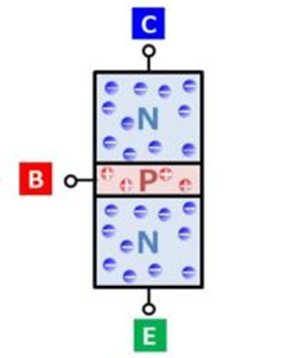
\includegraphics[height=32mm]{transistor_npn_structure.png}\hspace{5mm}
  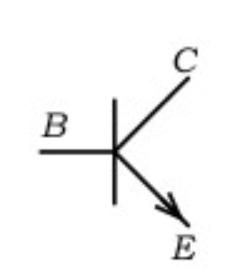
\includegraphics[height=24mm]{transistor_npn_symbol.png}
  \captionof{figure}{バイポーラトランジスタ（BJT）}
  \label{fig:transistor-bjt}
\end{center}
BJTは，ベース（B），コレクタ（C），エミッタ（E）の3つの端子を持つトランジスタです（\cref{fig:transistor-bjt}）。
ベースに流す小さな電流によって，コレクタとエミッタの間に流れる大きな電流を制御することから，「\important{電流で電流を制御する素子}」と考えることができます。
小さな入力に対して大きな電流変化を得やすく，音声信号やセンサ信号などを扱うアナログ増幅回路で用いられることが多いトランジスタです。
また，小型モータの駆動や速度制御などにも利用されます。
\end{tcolorbox}
\end{minipage}\hfill
\begin{minipage}[t]{0.49\linewidth}
\begin{tcolorbox}[enhanced, equal height group=transistor-types, colback=white, colframe=EGMain,
    boxrule=0.6pt, arc=1mm, left=2mm, right=2mm, top=2mm, bottom=2mm,
    fonttitle=\sffamily\gtfamily\bfseries, toptitle=1mm, bottomtitle=1mm,
    coltitle=white, colbacktitle=EGMain, title={電界効果トランジスタ（FET）}]
\begin{center}
  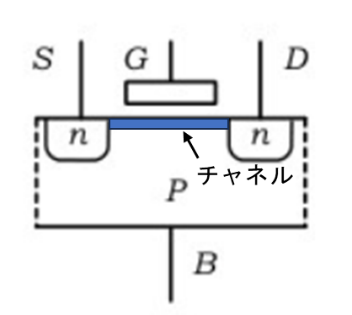
\includegraphics[height=32mm]{transistor_fet_structure.png}
  \captionof{figure}{電界効果トランジスタ（FET）}
  \label{fig:transistor-fet}
\end{center}
FETは，ゲート（G），ドレイン（D），ソース（S）の3つの端子を持つトランジスタです（\cref{fig:transistor-fet}）。
ゲートに加える電圧によって，ドレインとソースの間に流れる電流を制御することから，「\important{電圧で電流を制御する素子}」と考えることができます。
入力側に流れる電流が非常に小さく，小型化や高集積化にも適していることから，CPUやメモリなどのデジタル回路に広く用いられています。
また，大きな電力を扱う電源回路のスイッチングにも多く利用されています。
\end{tcolorbox}
\end{minipage}

% ------------------------------------------------------------
\subsection{バイポーラトランジスタの基本的な性能}

本実験ではBJTを扱っていきます。BJTは主にPNP型とNPN型があり，ここではNPN型について説明します。NPN型のトランジスタは，\cref{fig:transistor-bjt}のような記号で表され，ベース（B）に小さな電流を流すことで，エミッタ（E）からコレクタ（C）へ流れる大きな電流を制御できる素子です。すなわち「小さい入力電流で大きな出力電流を操る」増幅作用を持ちます。

NPN型では，ベース-エミッタ間に電圧（約\SI{0.7}{V}以上）を与えると，エミッタからベースへ電子が流れ込みます。ベースは非常に薄いため，その電子の一部のみが正孔と再結合してベース電流となり，残りのほとんどの電子はそのままコレクタへ引き抜かれます（コレクタ電流）。この結果，小さなベース電流に対して大きなコレクタ電流が流れます。この関係は $I_\mathrm{C}=\beta I_\mathrm{B}$（$\beta$ は電流増幅率）で表され，$\beta$ は一般に数十から数百の値をとります。また，コレクタ-エミッタ間に適切な電圧を与えることで，トランジスタはアナログ信号の増幅素子としてだけでなく，デジタル回路におけるスイッチとしても利用されます。

% ------------------------------------------------------------
\subsection{エミッタ接地増幅回路}

\begin{figure}[htbp]
  \centering
  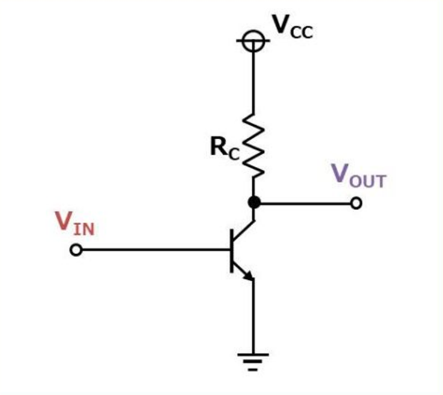
\includegraphics[height=45mm]{transistor_ce_amplifier.png}
  \caption{エミッタ接地増幅回路}
  \label{fig:transistor-ce}
\end{figure}

エミッタ接地増幅回路は，エミッタ端子を接地（GND）に接続し，ベースに直流電圧を加えてコレクタ電流を制御する回路です（\cref{fig:transistor-ce}）。ベース−エミッタ間にはおよそ\SI{0.7}{V}程度の電圧が必要であり，このとき流れるベース電流に比例してコレクタ電流が流れます。コレクタ電流が大きくなるとコレクタ抵抗にかかる電圧降下も大きくなり，その結果コレクタ電圧（$V_\mathrm{OUT}$）は低下します。このように入力側のベース電圧を変化させると，出力側のコレクタ電圧が反対方向に変化するため「反転動作」と呼ばれます。直流の実験では，この電圧−電流関係やコレクタ電圧の変化を測定し，トランジスタの基本特性と動作点の決まり方を確認できます。

% ============================================================
\section{実験}

結果は，ワークシートに記入してください。

% ------------------------------------------------------------
\subsection{実験1：乾電池（小さな入力信号）を用いてファンを回そう！}

\begin{equipment}[準備物]
ブレッドボード，ジャンパー線，ファン（\SI{12}{V}），乾電池（\SI{1.5}{V}），電池BOX，DCジャック，トランジスタ，ACアダプタ（\SI{12}{V}），抵抗（\SI{1}{k\ohm}）
\end{equipment}

\begin{figure}[htbp]
  \centering
  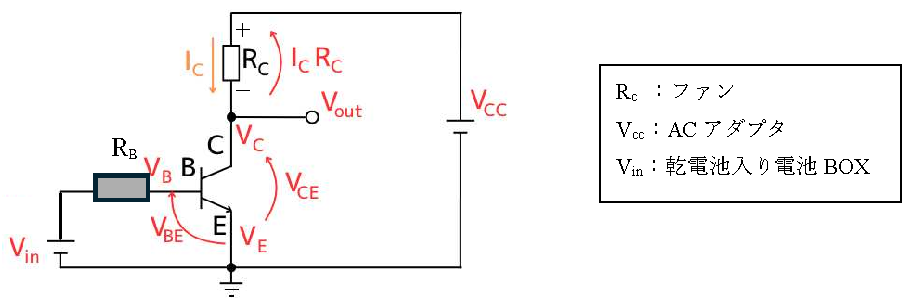
\includegraphics[width=0.95\linewidth]{transistor_fan_circuit.pdf}
  \caption{ファン駆動用エミッタ接地増幅回路}
  \label{fig:transistor-fan}
\end{figure}

\begin{figure}[htbp]
  \centering
  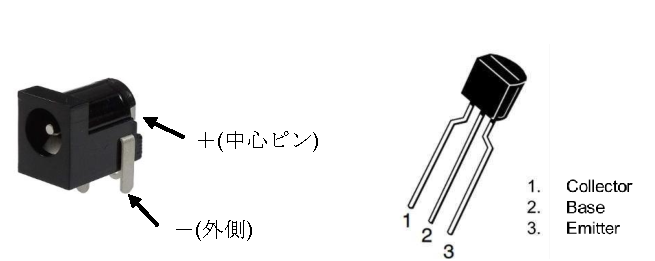
\includegraphics[width=0.7\linewidth]{transistor_dcjack_pinout.pdf}
  \caption{本実験で使用するDCジャックとトランジスタ}
  \label{fig:transistor-dcjack}
\end{figure}

\begin{procedure}[label=\textbf{1.\arabic*}, ref=1.\arabic*, leftmargin=*, labelsep=0.8em]
  \item ブレッドボード上で，乾電池入り電池BOXとファンを直列に接続し，ファンが駆動するか確認します。回ったかどうかをワークシートに記入してください。
  \item 乾電池でファンを回してみます。\cref{fig:transistor-fan}の回路図のように，ブレッドボード上に増幅回路を組み立てます。このときの $R_\mathrm{c}$ はファン，$V_\mathrm{cc}$ はACアダプタ，$V_\mathrm{in}$ は乾電池入り電池BOXです。\wave{トランジスタのエミッタ，コレクタ，ベースの各端子，およびDCジャックの極性（$+$・$-$）を，\cref{fig:transistor-dcjack}を参考にして正しく接続します。}
  \item 接続を確認した後，電池BOXのスイッチをオンにし，増幅回路を用いてファンを駆動します。\wave{ファンが回転したら教員の確認を受け}，実験2に進みます。
\end{procedure}

% ------------------------------------------------------------
\subsection{実験2：電圧−電流の関係やコレクタ電圧の変化を測定しよう！}

\begin{equipment}[準備物]
ブレッドボード，ジャンパー線，ファン（\SI{12}{V}），DCジャック，トランジスタ，ACアダプタ（\SI{12}{V}），抵抗（\SI{1}{k\ohm}×2個），直流電源，テスター
\end{equipment}

\begin{procedure}[label=\textbf{2.\arabic*}, ref=2.\arabic*, leftmargin=*, labelsep=0.8em]
  \item ファンが回り始める入力電圧のしきい値を確認します。増幅回路の入力電圧源 $V_\mathrm{in}$ を乾電池から直流電源に変更します。$V_\mathrm{in}$ を\SI{0}{V}から\SI{1.0}{V}まで\SI{0.05}{V}ずつ上昇させ，ファンが回り始めたときの電圧をワークシートに記録します。
  \item \label{item:transistor-graph} ファンを\SI{1}{k\ohm}のコレクタ抵抗 $R_\mathrm{c}$ に置き換え，抵抗の両端電圧 $V_{R_\mathrm{c}}$ をテスターで測定します。$V_\mathrm{in}$ を\SI{0}{V}から\SI{1.0}{V}まで\SI{0.05}{V}ずつ変化させ，横軸を $V_\mathrm{in}$，縦軸を $V_{R_\mathrm{c}}$ としてグラフを作成します。
  \item 出力電圧 $V_\mathrm{OUT}$ を，コレクタ端子とGNDとの間の電圧として測定します。$V_\mathrm{in}$ を\SI{0}{V}から\SI{1.0}{V}まで\SI{0.05}{V}ずつ変化させ，横軸を $V_\mathrm{in}$，縦軸を $V_\mathrm{OUT}$ として，\ref{item:transistor-graph}で作成したグラフ上にプロットします。
\end{procedure}
